\section{Box-office Predicting}
Movie box office is influenced by many factors, such as investment budget, script, director, actor, post production, producer and producer, media publicity and movie reputation. On the whole, we quantify the factors that affect movie box office from the film itself, the director, the actor and the audience. The opening week due to the lack of effective comments, so just for the release of the film at the box office during the period of life prediction problem, we consider the factors associated with the film at the box office and did not join the historic influence of sentiment analysis, in the opening week after we join in the model of the value of emotional factors.

\label{sec:predict}
\subsection{Premiere week box-office predicting}
\begin{table}[!htb]
  \centering
\begin{tabular}{|c|c|}
\hline
Symbol&Description\\
\hline
$sc$ &The mean $bos$ of famous creators\\
\hline
$gsc$&The mean $wms$ of famous creators\\
\hline
$std$&The variance $bos$ of famous creators\\
\hline
$gstd$&The variance $wms$ of famous creators\\
\hline
$starcounts$& The number of famous creators\\
\hline
$schedule$ & The schedule that the movie came out\\
\hline
$year$ & The year that the movie came out\\
\hline
\end{tabular}
  \caption{Features}
\label{tab:feature}
\end{table}
\par Table \ref{tab:feature} shows the features we used in the task of predicting premiere week box office. As is metioned above, the box office of a movie depends on not only movie factors itself including actors, directors, type, movie propaganda and so on but also influenced by audience reations. In addition, the time the movie released also has a certain impact on the movie box office. In general, predicting premiere week box-office can capture the influences of famous creators(actors and directors) to the movie. We provide Premiere week box-office predicting by using traditional box-office predicting model Support Vector Regression. This Module can help people to asses the influence of stars in the movie.

\subsection{Phased Box-office Predicting}
\begin{figure}[!htbp]
\centering
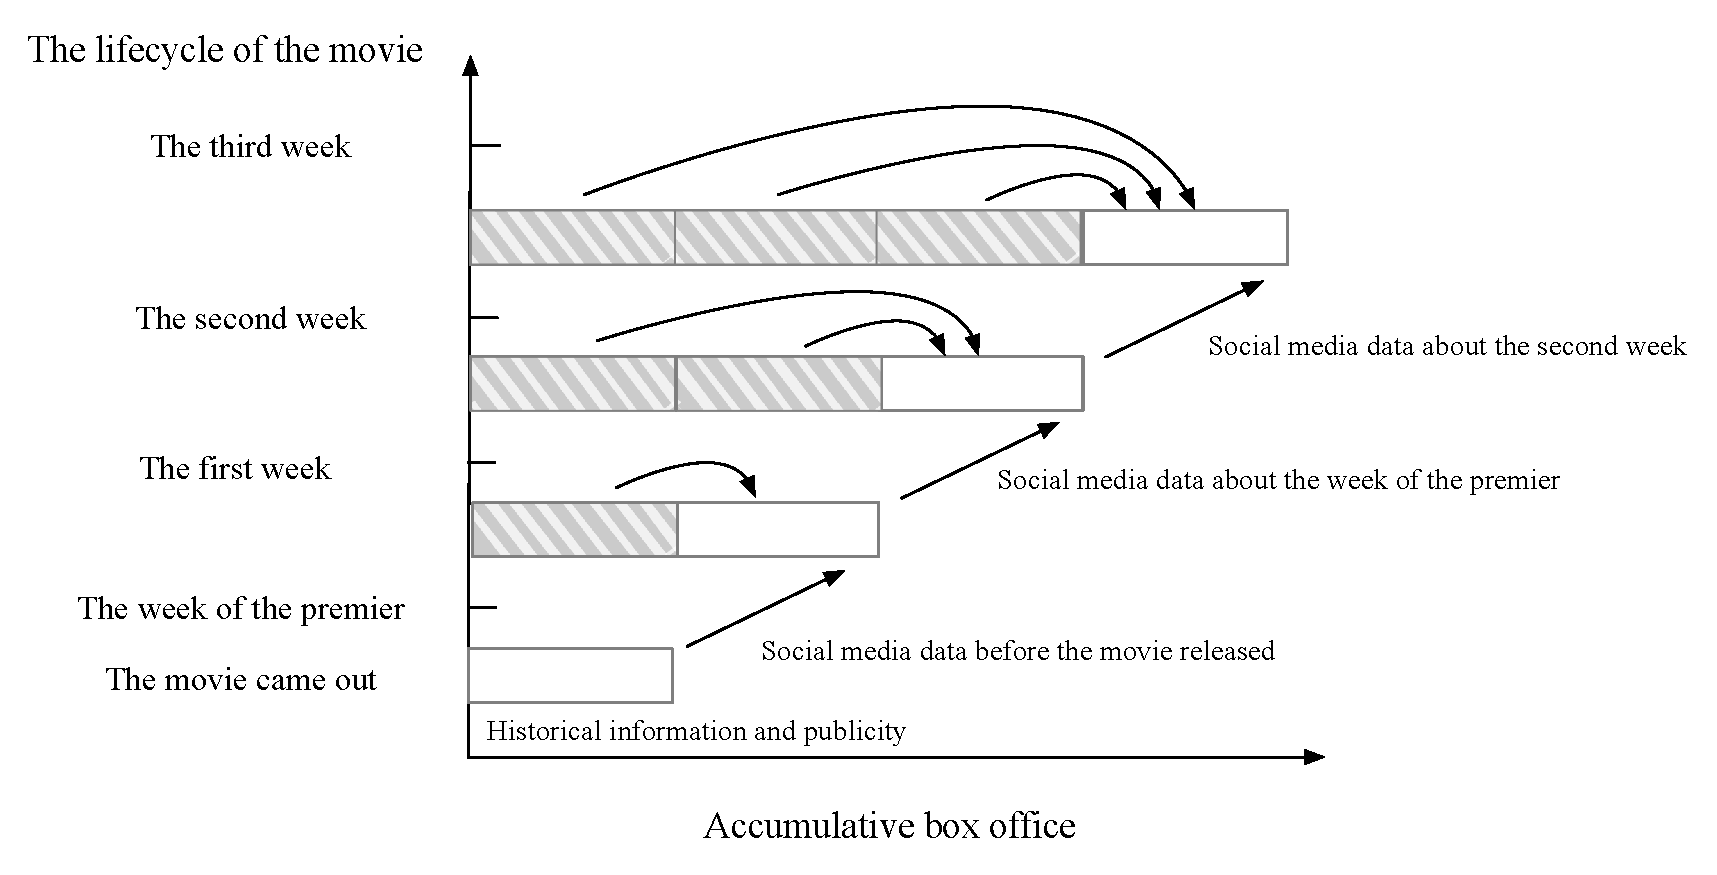
\includegraphics[width=0.8\columnwidth]{boxpredict.eps}
\caption{Multi-stage box office prediction model}
\label{fig:dyna}
\end{figure}
In the past prediction of box office, we usually only forecast the overall box office, but often ignored the movie's influence on movie box office due to the audience's attitude. Such as "wolf 2", the movie box office to be among the world's top 100, because in the release process, because the audience warmly, attracted the audience is not the original film (film series the fans, fans, like the kind of audience) to watch a movie, which leads to the box office continued to rise however, the traditional model is unable to capture this phenomenon. Therefore, as shown in Figure \ref{fig:dyna}, from the pre launch to the 1 months after the release, we set up the box office prediction model with the weekly variation of the weekly release to predict the box office for the first week, the box office for second weeks, the third week box office and the box office at the fourth week.
\par In this section, we add two type features: $weibo_i$, The ratio of creative comments and all comments until the $ith$ week
and $week_i$ The box office in the $ith$ week. With these additional messages obtained from audience and current box office, the results we predict are more similiar to real box office, shown in Table 3.
\begin{table*}[!htbp]
\centering
\begin{tabular}{|c|c|c|c|c|c|c|}
 \hline
    \multicolumn{1}{|c|}{\textbf{}}&
    \multicolumn{1}{|c|}{\textbf{\large Metric}}&
    \multicolumn{5}{|c|}{\textbf{\large Model}} \\
 \hline
    Week & Metric & SVR &  RF &  GBDT &  LR & LASSO\\
 \hline
    \multirow{3}{*}{\begin{sideways}{First}\end{sideways}}
    & MSE  & \textbf{0.09393658} &  0.2683265 & 0.6354384 & 1.09512416 & 0.74275155  \\
    & R2score & \textbf{0.63495534} &  -1.8019927	& -2.1466284 & -3.5673886 & -2.0977628   \\
    & EVC  & \textbf{0.6082226} & 0.4194317 & 0.20241852 & -3.0608791 & -0.9281806   \\
 \hline
     \multirow{3}{*}{\begin{sideways}{Second}\end{sideways}}
    & MSE  & 0.2716661 & 0.3192046 & 0.51210881 & 0.51052539 & \textbf{0.05284060}  \\
    & R2score & 0.0693802 & -1.0037243 & -0.78307969 & -0.74885631 & \textbf{0.81898915}   \\
    & EVC  & 0.1977912 & -0.1190541 & -0.08409798 & -0.69472796 & \textbf{0.91647358}   \\
 \hline
     \multirow{3}{*}{\begin{sideways}{Third}\end{sideways}}
    & MSE  & 0.3949564 &1.0082170 &0.764787 &0.73353798 &\textbf{0.0896601506}  \\
    & R2score & 0.6605046 &0.0296122 &0.297479 &0.369467937 &\textbf{0.9229302356}   \\
    & EVC  & 0.713641 &0.0253357 &0.611827 &0.37283487 &\textbf{0.9758343006}  \\
 \hline
      \multirow{3}{*}{\begin{sideways}{Forth}\end{sideways}}
    & MSE  &0.745514&0.6839145&2.03964614&1.373235192&\textbf{0.5025655348}  \\
    & R2score &0.573410&0.1461468&0.16642220&0.214224192&\textbf{0.7124281104}   \\
    & EVC  &0.63220&0.4586132&0.05054086&0.325419958&\textbf{0.7183931246}  \\
 \hline
\end{tabular}
\caption{Evaluation of Predicting Model}
\label{tab:evalution}
\end{table*}